\section{System Overview} Havven is designed to provide a decentralised currency with price stability. To achieve this, Havven implements two tokens and a unique price stabilisation mechanism. The first token is the Havven token, referred to as \HAV{} to avoid confusion with the system itself. \HAV{} serves two functions:

\begin{enumerate}
\item{To provide the system with collateral.}
\item{To allow actors to contribute to the process price stabilisation process and be rewarded for their efforts.}
\end{enumerate}

\noindent The second token is the Nomin, which will be referred to primarily as the \NOM{}, to remain consistent with \HAV{}. The goal of Havven is to maintain a constant \NOM{} price of \$1. In addition to providing collateral for the system, owners of the \HAV{} token are incentivised to maintain a level of supply in the \NOM{} market such that the market price remains constant. \\

\noindent Before continuing, we first introduce some basic system variables:

\begin{align*}
H &= \text{Quantity of \HAV{},} & N &= \text{Quantity of \NOM{},} \\
P_h &= \text{\HAV{} Price,}  & P_n &= \text{\NOM{} Price.}
\end{align*}

\noindent All \HAV{} tokens are created in the initial system state, so $H$ is a constant value. The quantity of \NOM{}, $N$ can float to ensure that the \NOM{} price, $P_n$ remains stable with changes in demand.

\subsubsection*{Price Stabilisation Rationale} Havven's approach to achieving price stability is to be passive where possible, intervening only when needed. To begin with, Havven leverages the utilisation ratio in order overcollateralize the Nomin, discussed in the next section. \\

\noindent Further, Havven provides economic incentives for \HAV{} holders to adjust the supply of \NOM{} when demand changes. In order to create these incentives, Havven charges fees when \NOM{} are transacted. These fees are redirected to the \HAV{} holders as a reward for maintaining the correct supply of \NOM{} . \\

\noindent Havven also benefits from a positive feedback loop for for small changes in $P_n$. A small decrease in $P_n$ should result in increased market demand, given the expectation of the return to \$1. 

\newpage

\subsection{Nomin Issuance} The only way \NOM{} can be issued is when a \HAV{} owner decides to escrow their \HAV{}. This ensures that there is always collateral backing a \NOM{} when it is issued. \\

\begin{namedthm}{Escrow}[]
To lock some quantity of \HAV{} in the system.
\end{namedthm}

\noindent When a Havven holder escrows their \HAV{}, the system will generate a quantity of \NOM{}. The system will then immediately place a limit sell order with a price of \$1 for on the Havven Decentralised Exchange. This means that the \NOM{} will be sold at market price, until the price reaches \$1 USD. The proceeds of this sale are then remitted to the issuer in ETH. It is important that the pool of \NOM{} is always overcollateralized by the value of \HAV{}. In order to achieve this, Havven must determine what is known as the utilisation ratio. \\

\begin{namedthm}{Utilisation Ratio}[]
$$ U = \frac{P_n * N}{P_h * H}. $$
\end{namedthm}

\noindent The utilisation ratio compares the total value of \NOM{} against the total value of \HAV{}. Intuitively if $U = 1$, the value of \NOM{} and \HAV{} are equal. Havven wants to be overcollateralised which means we would like to maintain $U <  1$. To do this, Havven only allows the issuance of \NOM{} up to a maximum utilisation ratio. \\

\begin{namedthm}{Havven Collateralisation Goal}[]
$$ 0 \leq U \leq U_{max} \leq 1.$$
\end{namedthm}

\noindent The maximum utilisation ratio is the first of Havven's price stabilisation mechanisms. It ensures that for every \NOM{}, there is a multiple of \HAV{} backing its value, escrowed in the system. \\

\noindent The issuance concept is best understood using an example:
\begin{enumerate}
\item{Bob owns 10 \HAV{} worth \$10 each, total value \$100.}
\item{The maximum utilisation ratio is 0.2.}
\item{Bob decides to escrow all of his \HAV{}, equivalent to 20 \NOM{}.}
\item{The system sells 20 \NOM{} on the market and transfers the proceeds, in eth to Bob's wallet.}
\item{Bob's \HAV{} are escrowed meaning he cannot use them in any way.}
\end{enumerate} 

\newpage

\noindent What If Bob wishes to retrieve his \HAV{} from escrow? He must burn the same the quantity of \NOM{} that was sold initially. \\

\begin{namedthm}{Burn}[]
To return \NOM{} to the system to be destroyed and release the \HAV{} that were escrowed. 
\end{namedthm}

\noindent In our example from before, Bob would need to burn the $20$ \NOM{} that he issued originally. \\

\noindent Likely some questions have already arisen: \\

\noindent \emph{1. Does Bob have to lock all of his \HAV{} into escrow?} \\ 

\noindent There is no requirement for Bob to escrow all of his \HAV{}, he can escrow as many as he likes. The quantity of \NOM{} that is sold on the market is $ P_h * H_e * U_{max} $ where $H_e$ indicates the quantity of \HAV{} that was escrowed. \\

\noindent \emph{2.What if Bob would like to release his \HAV{}? Where would he acquire \NOM{}?} \\ 

\noindent He simply needs to buy some more in the open market. \HAV{} and \NOM{} are both ERC20 tokens that will be traded on a variety of centralised and decentralised exchanges. Once he buys $20$ \NOM{}, he can present them to the system to be burned, thus releasing the escrowed \HAV{} back to him. \\ 

\noindent \emph{3. What happens if the price of \HAV{} has changed?} \\

\noindent All issuance of \NOM{} is done at the current $P_h$. However, $P_h$ is determined by the market (or by target price ratio TBA). This means when $P_h$ changes, the quantity of escrowed \HAV{} changes with it. An increase in $P_h$ means that fewer of Bob's \HAV{} are escrowed. In contrast, a decrease in the $P_h$ means that more of his \HAV{} are escrowed. This process occurs automatically in order to ensure that the system remains overcollateralised. \\ 

\noindent \emph{4. What happens if the price of \NOM{} has changed?} \\ 

\noindent In order to release escrowed \HAV{} the Bob must return the same quantity of \NOM{} that he issued. This means that if $P_n$ has increased in the market, he will need to spend more Eth than he received when he issued the \NOM{} in order to release his \HAV{}. In contrast, if $P_n$ has decreased, the user will need to spend less Eth in order to release his \HAV{}.

\newpage

\subsection{Nomin Demand and Supply} 

\noindent Demand and supply economics shows that there exists some optimal supply of \NOM{} where the related level of demand yields an equilibrium price of \$1. We can express this quantity in terms of the utilisation ratio, $U_{opt}$. The graph below visualises this situation. \\

\begin{figure}[h!]
    \centering
    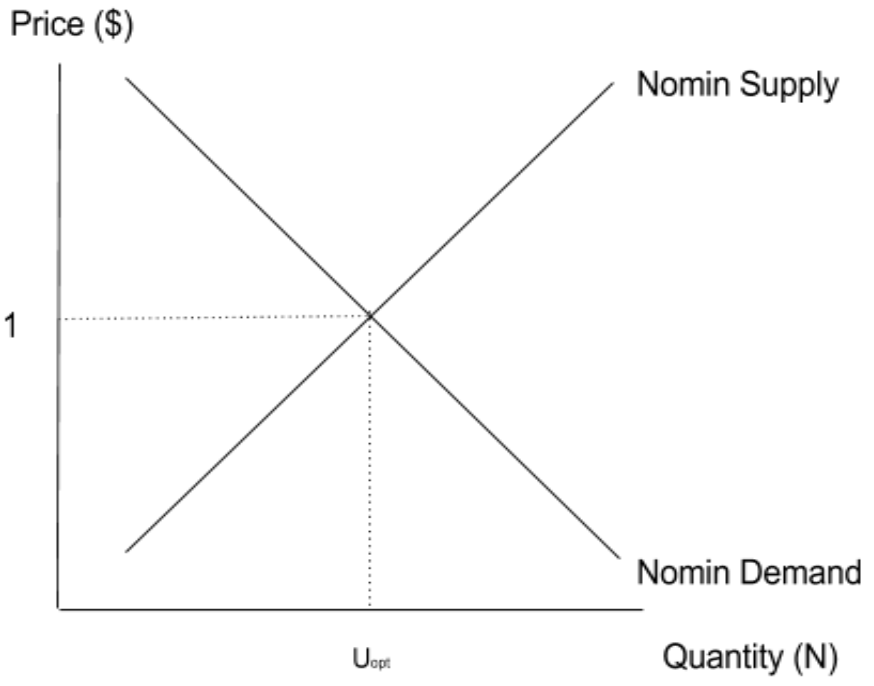
\includegraphics[width=.7\textwidth]{img/nomin-demand-vs-supply}
\end{figure}

\subsubsection*{Demand}

\noindent The system is unable to influence the demand for \NOM{}. It will come primarily from the utility of a stable Nomin.

\subsubsection*{Supply}

\noindent However, the supply of \NOM{} is controlled directly by the Havven holders, who use the system to issue and burn \NOM{}. This means the system can provide incentives for Havven holders to expand and contract the \NOM{} supply when demand changes. \\

\noindent The goal of Havven is to incentivise the Havven holders to maintain the level of \NOM{} supply at $U_{opt}$, such that $P_n = 1$. In order to do this, the system must provide incentives to the \HAV{} token holders.  \\

\newpage

\subsection{Transaction Fees} Every time a Nomin transaction occurs, the Havven system charges a small transaction fee. Transaction fees allow the system to generate revenue, which it can distribute to \HAV{} holders as an incentive to maintain \NOM{} supply at $U_{opt}$. \\

\begin{namedthm}{Fees Charged (per transaction)}[]
$$ a_c = k.$$
\end{namedthm}

\noindent The fee charged on Nomin transactions is constant and will be sufficiently small that it provides little to no friction for the user. \\

\begin{figure}[h!]
    \centering
    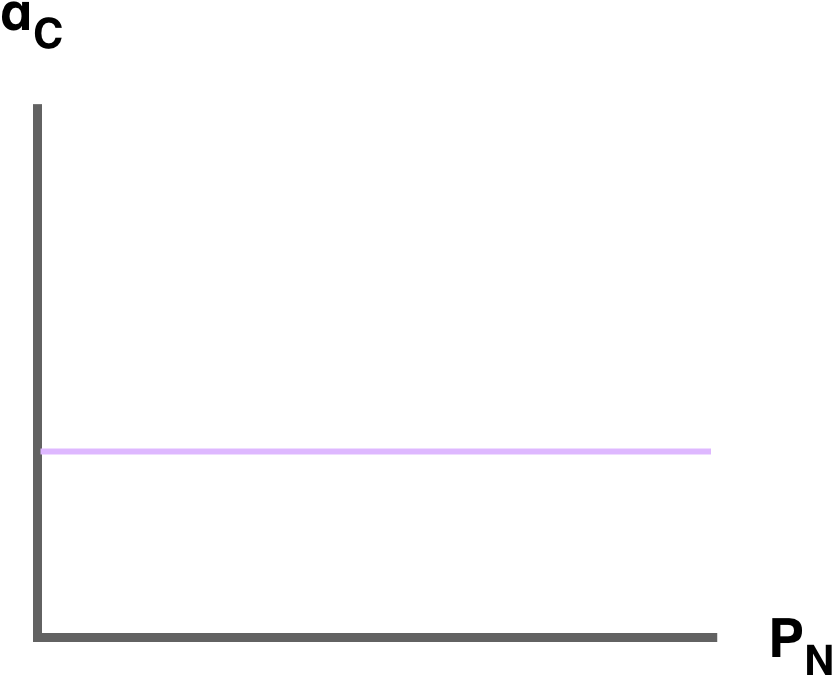
\includegraphics[width=.55\textwidth]{img/fees-charged}
\end{figure}

\newpage

\begin{namedthm}{Fees Received (per escrower)}[]
\[
\alpha_r = 
\begin{cases}
 \frac{\alpha_{base}}{U_{opt}} * U_I &\mbox{when } U_I \leq U_{opt}, \\ 
 \frac{\alpha_{base}}{U_{max} - U_{opt}} * (U_I  - U_{max}) &\mbox{when } U_{opt} \leq U_I \leq U_{max}, \\ 
 0 &\mbox{otherwise}.
 \end{cases}
\]
\end{namedthm}

\begin{figure}[h!]
    \centering
    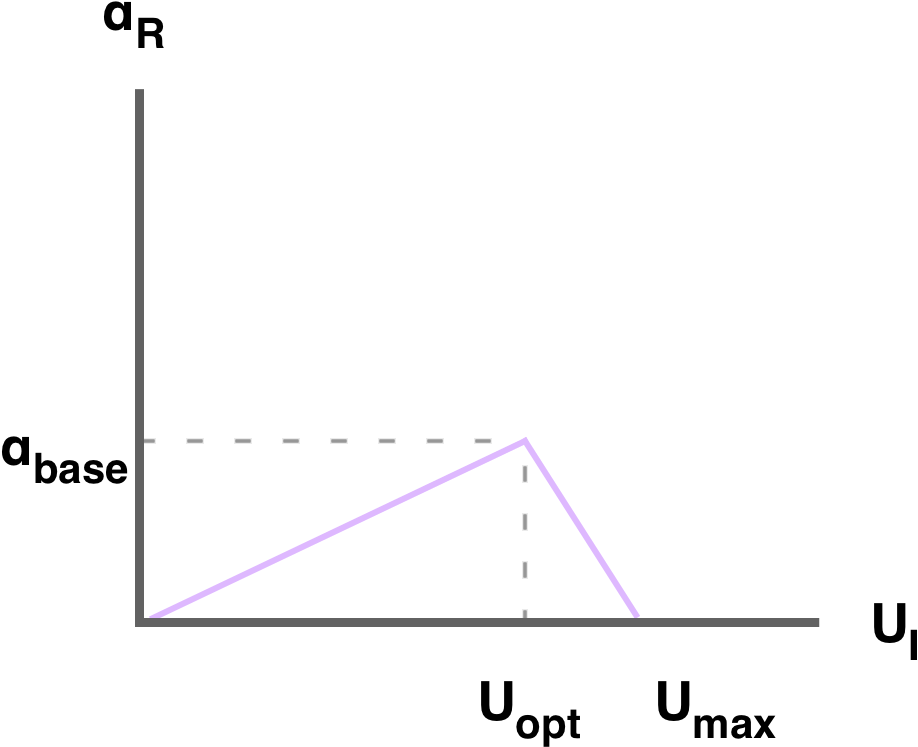
\includegraphics[width=.55\textwidth]{img/fees-received}
\end{figure}

\noindent Fees are only paid to \HAV{} holders who have elected to escrow, as a reward for collateralising the system. The fees received increases linearly to a maximum at the optimal utilisation ratio $U_{opt}$. However, the fees quickly diminish as $U_I$ approaches $U_{max}$ and drop to nothing after this point. \\

\noindent Intuitively, this equation encourages \HAV{} holders who have escrowed to maintain their $U_I$ at $U_{opt}$. 

\newpage

\noindent Recall the concept of the utilisation ratio, which was introduced earlier:

$$ U = \frac{P_n * N}{P_h * H}. $$ \\

\noindent We have introduced the concept of an optimal utilisation ratio and its importance in achieving Havven's  goal $P_n = 1$. Havven's fee structure encourages all \HAV{} holders who escrow to maintain their personal utilisation ratio $U_I$ at $U_{opt}$. However, the system needs a function to determine what $U_{opt}$ is. \\

\noindent If $P_n > 1$ then the system must encourage more \NOM{} to be issued. If $P_n < 1$ the system must encourage \NOM{} to be burned. The definition of $U_{opt}$ must provide this incentive. \\

\begin{namedthm}{Optimal Utilisation Ratio}[]
$$ U_{opt} = f(P_n) * U,$$
$$ f(x) = max(\sigma * (x - 1)^{\phi} + 1, 0), $$
$$\text{where } 0 \leq \sigma, \text{ the price sensitivity parameter}, $$
$$\phi \geq 1, \text{ the flattening parameter}. $$
\end{namedthm}

\begin{figure}[h!]
    \centering
    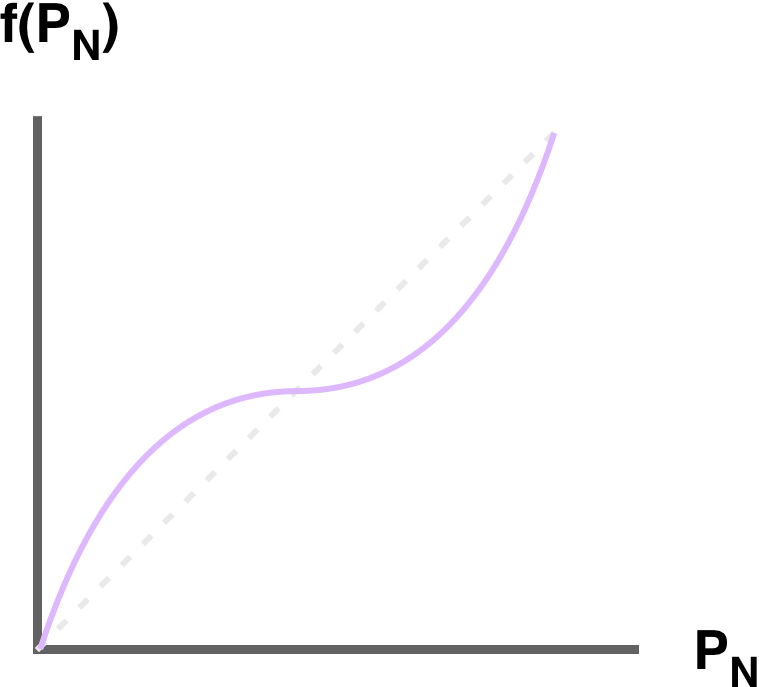
\includegraphics[width=.5\textwidth]{img/U_opt}
\end{figure}

\noindent The graph above shows that the when $P_n$ is near \$1, f'(x) is small. However, the further $P_n$ diverges from \$1, the larger the derivative becomes. This means the incentive to move toward $U_{opt}$ increases as $P_n$ diverges from \$1.

\newpage

\subsection*{Maximum Utilisation Ratio}

\noindent When we discussed the concept of issuing \NOM{}, we introduced the idea of a maximum utilisation ratio, $U_{max}$. Havven needs to maintain $U < U_{max} < 1$, in order to remain overcapitalised. It might seem intuitive that $U_{max}$ should be a static value. However, since $U_{opt}$ changes linearly with $P_n$ and inversely with $P_h$, there are several situations where $U_{max}$ may need to change. Below we define $U_{max}$.

\begin{namedthm}{}[]
\[
U_{max} = 
\begin{cases}
 U_{base} &\mbox{when } U_{opt} \leq U_{base}, \\ 
 \alpha * U_{opt} &\mbox{otherwise}.
 \end{cases}
\]
\end{namedthm}

\begin{figure}[h!]
    \centering
    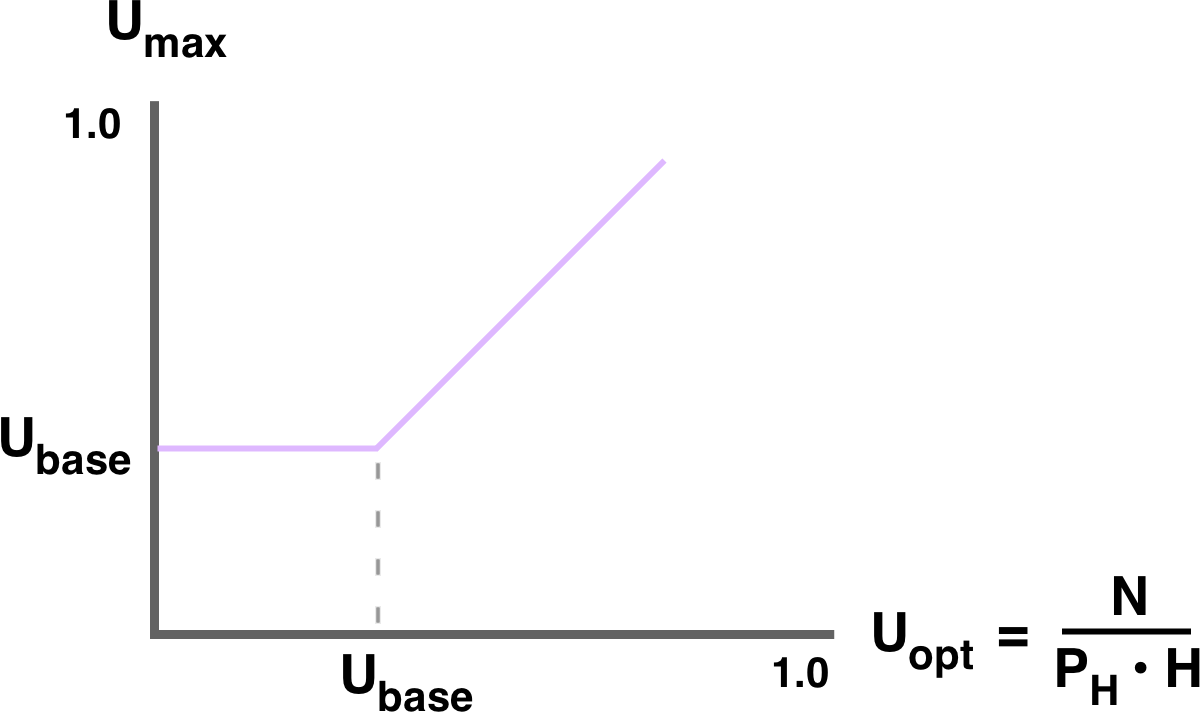
\includegraphics[width=.75\textwidth]{img/U_max}
\end{figure}

\newpage

\subsection{Intrinsic Havven Price} With the \HAV{} token being ERC20 compliant, it will have a market price on both decentralised and centralised exchanges. \\

\noindent While the system will access the market price via an oracle, it is also beneficial to define a $P_h$ that can be determined internally, thus avoiding the impact of speculation. Ignoring speculative demand, $P_h$ can be expressed as a function of the transaction fees that the system charges. Below we define an initial iteration of the intrinsic $P_h$.

\begin{namedthm}{Havven Price}[]
\begin{align*} 
P_{h,t} &= \frac{1}{H}* \sum\limits_{t=1}^\infty \frac{d_{n,t} *v_{n,t} * \alpha_{R,t}}{(1+R)^t} \approx \frac{d_{n,t} *v_{n,t} * \alpha_{R,t}}{R * H}, \\
& P_{h,t} \text{ is the price of one \HAV{} at time } t, \\
& H \text{ is the number of havvens}, \\
& d_{n,t} \text{ is the demand for \NOM{} at t}, \\
& v_{n,t} \text{ is the velocity of \NOM{} at t}, \\
& \alpha_{R,t} \text{ is the fee from trade with \NOM{}}, \\
& R \text{ is the interest rate / rate of return of havvens}. \\
\end{align*}
\end{namedthm}

\newpage

\subsection{Juans Description of Players (Refactored)}
\begin{namedthm}{Havven Holder}[]
An investor who owns \HAV{} tokens.
\end{namedthm}

\noindent In order to purchase \HAV{} the expected return has to be greater than that of alternative investments (opportunity cost). The expected return of \HAV{} comes from:
\begin{enumerate}
\item{The fees received on escrowed \HAV{}.}
\item{An increase in $P_h$.}
\item{Seigniorage (i.e., an increment in $P_h$ implies that the investor can issue more \NOM{}, which may eventually have a larger value than his original investment.}
\end{enumerate}

\noindent At any moment in time, the investor must decide:
\begin{enumerate}
\item{Whether or not to issue new \NOM{} (assuming $U_I < U_{max}$), or to burn some of them. All \NOM{} are issued/burnt at the prevailing market exchange rate, denominated in ETH.}
\item{Whether to sell some quantity of \HAV{} in the market at price $P^M_{h,t}$. Only \HAV{} which haven't been escrowed can be sold. Otherwise they must burn \NOM{} to release them. }
\end{enumerate}

\begin{namedthm}{Nomin User}[]
A person who uses the Nomin token.
\end{namedthm}
 
\noindent In order to purchase \NOM{}, it must provide the user more utility than USD, since both have the same consumption value in the market. This utility may come from the properties of crypto. \\

\noindent At any time, they must decide: 
\begin{enumerate}
\item{Whether to buy or to sell \NOM{} at $P_n$.}
\end{enumerate}

\newpage